%---------------------------------------------------------
% Chapter: A chapter about grahics
%----------------------------------------------------------
\chapter{Creating and Including Graphics}
\label{chap:GRAPHICS}

They say a picture is worth 1000 words.  That is probably true of a
good picture, but you don't want to go overboard with pictures just to
fill up space.  After a while, your readers will catch on to the scam
you are trying to perpetrate.

Before we discuss how to do get pictures, graphs, and other graphical
items into a \LaTeX\ document, a tiny bit of background will be useful.

\section {Types of Graphics}

There are essentially two types of graphics you can include: bitmaps
and vector graphics.  Bitmaps are found in files with extensions such
as \verb|.jpeg|, \verb|.png|, \verb|.gif|, and the laughably horrid
\verb|.bmp|.  In bitmap images, the information has already been
chopped up into individual units called pixels.  When you show a
bitmap image on the screen, or print a bitmap image on a printer, if
there is not an exact one-to-one correspondence between the image
pixels and the output device pixels, the image has to be scaled up or
down, which typically reduces the quality of the image and gives poor
results.  You can not always avoid these image types, but it is a good
idea to avoid them whenever possible.

The compression used in \verb|.jpeg| files is designed for
photographic (and similar) images, and does not work well for line
drawings or textual material.  If you must use a bitmap image, use
JPEGs for photos and PNGs for other material.

Unlike bitmap images, vector graphics are lists of ``instructions''
telling the displaying program where to draw lines, curves and points.
Typically these will scale up and down very well, and therefore these
are usually a much better choice than bitmap graphics.  For X-Y plots
(for example), you should use some tool which creates vector graphics,
if at all possible.

The inventor of \TeX\ (Donald Knuth) made a conscious decision to NOT
include graphics features directly into \TeX.  He knew that such an
approach would be doomed to failure, since better, more convenient
graphics facilities would be created in the future.  But he realized
that graphics are important, so \TeX\ has a feature to allow graphics
from other systems to be included.  More recently some people have
designed add-on packages to \TeX\ and \LaTeX\ which gives you some
powerful graphics capabilities from within \TeX\ and \LaTeX.  Some
examples are shown below.


\section {Including External Graphics}
\label{sec:IEG}

If you have created a graphic which you want to include in your
thesis, assuming you have \verb|\usepackage{graphicx}| in (for
example) your header file, you can then type
\begin{center}
    \verb|\includegraphics[width=WIDTHOFGRAPHIC]{GRAPHIC_LOCATION}|
\end{center}
Note that the \verb|[width=WIDTHOFGRAPHIC]| option adjusts
the width of the graphic to be \verb|WIDTHOFGRAPHIC| in the 
document.  For example, \verb|[width=0.80\textwidth]| will
set the width to be $80\%$ of the width of the text at that 
point in the document.  You could also write \verb|width=5in| to make
the graphic exactly 5 inches wide.  (There is also a
\verb|[height=...]| option, should that be more convenient for you.)

The code
\begin{verbatim}
\begin{center}
    \includegraphics[width=.50\textwidth]{figures/example}
\end{center}
\end{verbatim}
produces the following image:

\need 2 in

\begin{center}
     \includegraphics[width=.50\textwidth]{figures/example}
\end{center}

This image looks rather lonely sitting there by itself.  Instructions
for attaching a figure number and a caption to such an image are found
in Chapter~\ref{chap:FIGURESANDTABLES}.

To show you why you should never, ever, ever use a bitmap image if you
have a vector graphics image available, here is an original vector
graphics image and the same image converted to a bitmap.  Need we say more?

\begin{center}
    \includegraphics[width=.4\textwidth]{figures/oven}
    \quad
    \includegraphics[width=.4\textwidth]{figures/oven-bitmap}  
\end{center}
%
(OK, one of us can't resist: ``Just don't do it''; ``Friends don't let
friends use bitmap images''; ``Just say no''.  Even if you think your
spreadsheet plot looks good on the screen, do not export it as a
bitmap or use a screen capture program to grab it.)

\subsection {Graphics File Types}

Unfortunately, \LaTeX\ can not use every type of graphics known.
Specifically, \verb|latex| can use encapsulated PostScript
(\verb|.eps|) files, and \verb|pdflatex| can use \verb|.png|,
\verb|.jpg|/\verb|.jpeg| and \verb|.pdf| files.

In the examples above, no file extension was explicitly used, which
means that \verb|latex| or \verb|pdflatex| will pick an appropriate
choice.  How this choice is made is left as a small research project
for the diligent student.

\section {Internal Graphics}

There are two very powerful add-on packages for \TeX\ and \LaTeX: PS
Tricks and TikZ/PGF.  PS Tricks is extremely powerful, but can only be
used (directly) with \verb|latex|; TikZ/PGF is also very powerful, and
can be used with both \verb|latex| and \verb|pdflatex|.

Unfortunately, both of these have a learning curve which is a bit
steep.  However, just to whet your appetite, here are a few
examples using TikZ/PGF.  Note that there are tutorials and
collections of samples to be found on the internet; for example, look
at \url{http://www.texample.net/tikz/examples/}
to see a gallery of sample figures produced using TikZ/PGF. 

Here is a sample of a log-log plot created with the following code:
\begin{verbatim}
  \begin{tikzpicture}
    \loglogaxis
    \addplot coordinates {
        (1,1)
        (16,16)
        (32,64)
    };
    \endloglogaxis
  \end{tikzpicture}
\end{verbatim}

\vspace{10pt}


\pgfplotsset{compat=1.3}% <-- moves axis labels near ticklabels (respects tick label widths)

\begin{tikzpicture}
    \loglogaxis
    \addplot coordinates {
        (1,1)
        (16,16)
        (32,64)
    };
    \endloglogaxis
\end{tikzpicture}

One of the nice things about using TikZ/PGF is that you don't have to
worry about external graphics files becoming separated from the rest of
your document when you move your files from one place to another.

Here is another slightly more complicated example:

\vspace{10pt}

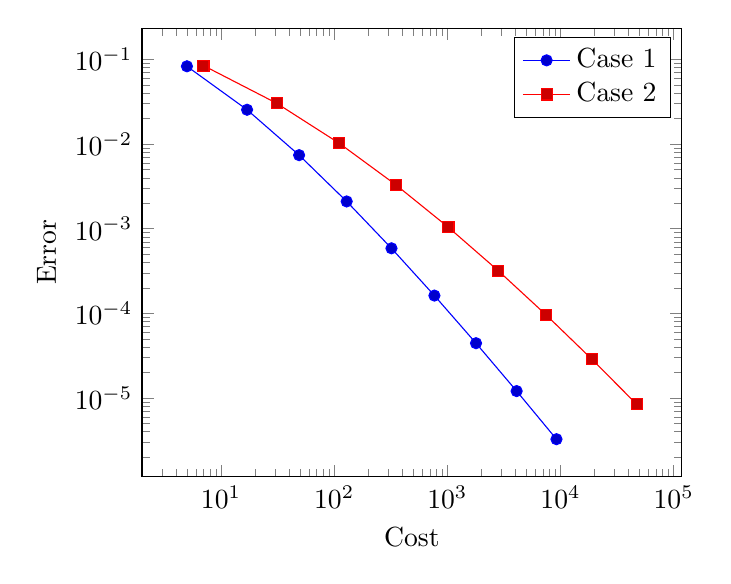
\begin{tikzpicture}
        \loglogaxis[
                xlabel=Cost,
                ylabel=Error]
        \addplot coordinates {
                (5,     8.31160034e-02)
                (17,    2.54685628e-02)
                (49,    7.40715288e-03)
                (129,   2.10192154e-03)
                (321,   5.87352989e-04)
                (769,   1.62269942e-04)
                (1793, 4.44248889e-05)
                (4097, 1.20714122e-05)
                (9217, 3.26101452e-06)
        };
        \addplot coordinates {
                (7,     8.47178381e-02)
                (31,    3.04409349e-02)
                (111,   1.02214539e-02)
                (351,   3.30346265e-03)
                (1023,  1.03886535e-03)
                (2815,  3.19646457e-04)
                (7423,  9.65789766e-05)
                (18943, 2.87339125e-05)
                (47103, 8.43749881e-06)
        };
        \legend{Case 1,Case 2}
        \endloglogaxis
\end{tikzpicture}


The code to produce that is the following:
\begin{verbatim}
  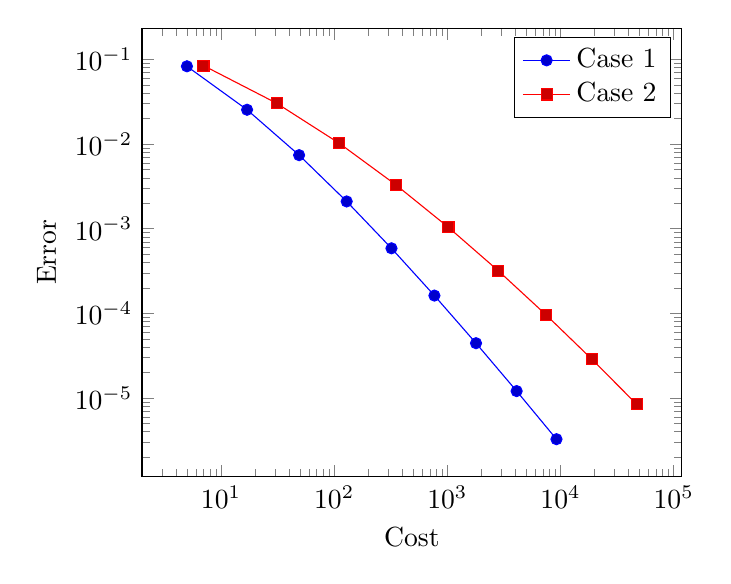
\begin{tikzpicture}
    \loglogaxis[
        xlabel=Cost,
        ylabel=Error]
    \addplot coordinates {
        (5,     8.31160034e-02)
        (17,    2.54685628e-02)
        (49,    7.40715288e-03)
        (129,   2.10192154e-03)
        (321,   5.87352989e-04)
        (769,   1.62269942e-04)
        (1793, 4.44248889e-05)
        (4097, 1.20714122e-05)
        (9217, 3.26101452e-06)
    };
    \addplot coordinates {
        (7,     8.47178381e-02)
        (31,    3.04409349e-02)
        (111,   1.02214539e-02)
        (351,   3.30346265e-03)
        (1023,  1.03886535e-03)
        (2815,  3.19646457e-04)
        (7423,  9.65789766e-05)
        (18943, 2.87339125e-05)
        (47103, 8.43749881e-06)
    };
    \legend{Case 1,Case 2}
    \endloglogaxis
  \end{tikzpicture}
\end{verbatim}

\medskip
As you can see, if you have large amounts of data, you might not want
to massage it into the format required for TikZ/PGF.

Aside from X-Y plots, TikZ/PGF is very nice for creating graphs such
as the following finite automaton:

\usetikzlibrary{automata}
\makeatletter
\def\tikz@double@width@distance{1.6pt}  % default 0.6
\makeatother

\begin{tikzpicture} [shorten >=1pt,>=stealth,node distance=3.5cm,auto]
    %\draw[help lines] (0,0) grid (3,2);
    \node[state,initial,accepting]     (q_0) {$q_0$};
    \node[state]                       (q_1) [right of=q_0] {$q_1$};
    \node[state,accepting]             (q_2) [right of=q_1] {$q_2$};
    \node[state]                       (q_3) [above of=q_1] {$q_3$};
    \path[->]
        (q_0) edge node {0} (q_1)
              edge [loop below] node {1} (q_0)
              edge node {$\epsilon$} (q_3)
        (q_1) edge node {$\epsilon$} (q_2)
              edge [loop below] node {0} (q_1)
        (q_3) edge [loop above] node {0,1} (q_3)
              edge node {1} (q_1);
\end{tikzpicture}


\medskip
That was produced with the following code:

\begin{verbatim}
\usetikzlibrary{automata}
\makeatletter
\def\tikz@double@width@distance{1.6pt}  % default 0.6
\makeatother

\begin{tikzpicture} [shorten >=1pt,>=stealth,node distance=3.5cm,auto]
    %\draw[help lines] (0,0) grid (3,2);
    \node[state,initial,accepting]     (q_0) {$q_0$};
    \node[state]                       (q_1) [right of=q_0] {$q_1$};
    \node[state,accepting]             (q_2) [right of=q_1] {$q_2$};
    \node[state]                       (q_3) [above of=q_1] {$q_3$};
    \path[->]
        (q_0) edge node {0} (q_1)
              edge [loop below] node {1} (q_0)
              edge node {$\epsilon$} (q_3)
        (q_1) edge node {$\epsilon$} (q_2)
              edge [loop below] node {0} (q_1)
        (q_3) edge [loop above] node {0,1} (q_3)
              edge node {1} (q_1);
\end{tikzpicture}
\end{verbatim}

One of the nice things about using a package like TikZ/PGF is that,
while there is a learning curve involved, and there is no
instantaneous visual feedback as when using a programs such as
\verb|xfig|, \verb|dia|, or (*gag*) \verb|visio|, there is also no
endless fussing trying to get the lines and circles arranged in a
visually pleasing, consistent manner.  For example, note that the
edges in the automaton graph all point to the centers of their
corresponding nodes, rather than just pointing to some random spot
on the edge of the node.

A second nice thing about using TikZ/PGF can be observed by reviewing
the figures in Section~\ref{sec:IEG}; the text in these figures does
not match the text in the rest of this chapter (both the typeface and
the size are wrong).  This is a recurring problem when you includes
figures or other graphics created using other programs.  Depending on
the program creating the figure, you may find it either difficult or
impossible to make the text consistent.  When possible, it is nice to
avoid this ugly-ism, and one way to do so is to use TikZ/PGF for your
graphics.

There is a \textbf{very} extensive user manual for this package; on a
Linux system run the command ``\texttt{texdoc tikz}'' to see the
documentation.

As a final example, in Figure~\ref{fig:SNARK} an example of a
(graph-theoretic) graph drawn using TikZ/PGF is shown; note that the
textual labels of the graph perfectly match the rest of the text.  If
you want to see the commands used to create Figure~\ref{fig:SNARK},
look in the \verb|graphics-info.tex| input file.  If you need to
perk your interest a bit more, look at
\url{http://www.texample.net/tikz/examples/} to see a gallery of
sample figures produced using TikZ/PGF.

\begin{figure}[ht]
  \centering
  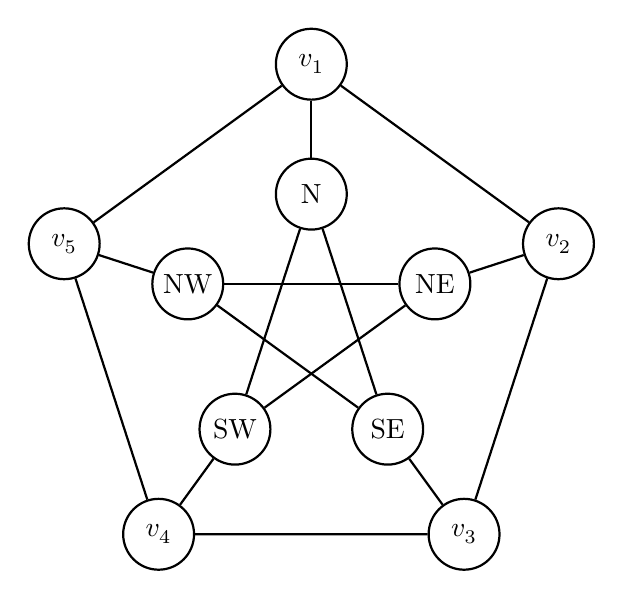
\begin{tikzpicture}[xscale=1.65,yscale=1.65,thick,
        nodeStyle/.style={shape=circle,minimum size=0.9cm,
            inner sep=0.2pt,draw},
        specialEdge/.style={ultra thick, dashed}]
% For unlabelled small or medium graphs the minimum node size
% looks better at something like 0.3 cm.
    \foreach \num/\theta/\r in {
        1/90/2, 2/18/2, 3/306/2, 4/234/2, 5/162/2}
    {
        \node (\num) at (\theta:\r) [nodeStyle] {$v^{}_{\num}$};
    }
    \foreach \num/\theta/\r/\text in {
            6/90/1/N, 7/18/1/NE, 8/306/1/SE, 9/234/1/SW, 10/162/1/NW}
    {
        \node (\num) at (\theta:\r) [nodeStyle] {\text};
    }
    \path \foreach \u/\v in {
        1/2, 2/3, 3/4, 4/5, 5/1,
        6/8, 7/9, 8/10, 9/6, 10/7, 1/6, 2/7, 3/8, 4/9, 5/10}
    {
        (\u) edge[] node {} (\v)
    };
  \end{tikzpicture}.
  \caption{The Petersen Graph.}
  \label{fig:SNARK}
\end{figure}

Aside from the matching text size and typeface in
Figure~\ref{fig:SNARK}, note the symmetry and precision of the
placement of the circles and the fact that the lines are positioned
exactly as they should be.  Learning a bit of TikZ/PGF to create
figures will take a while, but it is worth it.  (Conversely, doing a
mediocre job with a GUI drawing program is easy, but doing something
worthy of your thesis using most GUI tools is much trickier.)
